\documentclass[14pt,xcolor=pdftex,dvipsnames,table]{beamer}\usepackage[]{graphicx}\usepackage[]{color}
%% maxwidth is the original width if it is less than linewidth
%% otherwise use linewidth (to make sure the graphics do not exceed the margin)
\makeatletter
\def\maxwidth{ %
  \ifdim\Gin@nat@width>\linewidth
    \linewidth
  \else
    \Gin@nat@width
  \fi
}
\makeatother

\definecolor{fgcolor}{rgb}{0.345, 0.345, 0.345}
\newcommand{\hlnum}[1]{\textcolor[rgb]{0.686,0.059,0.569}{#1}}%
\newcommand{\hlstr}[1]{\textcolor[rgb]{0.192,0.494,0.8}{#1}}%
\newcommand{\hlcom}[1]{\textcolor[rgb]{0.678,0.584,0.686}{\textit{#1}}}%
\newcommand{\hlopt}[1]{\textcolor[rgb]{0,0,0}{#1}}%
\newcommand{\hlstd}[1]{\textcolor[rgb]{0.345,0.345,0.345}{#1}}%
\newcommand{\hlkwa}[1]{\textcolor[rgb]{0.161,0.373,0.58}{\textbf{#1}}}%
\newcommand{\hlkwb}[1]{\textcolor[rgb]{0.69,0.353,0.396}{#1}}%
\newcommand{\hlkwc}[1]{\textcolor[rgb]{0.333,0.667,0.333}{#1}}%
\newcommand{\hlkwd}[1]{\textcolor[rgb]{0.737,0.353,0.396}{\textbf{#1}}}%

\usepackage{framed}
\makeatletter
\newenvironment{kframe}{%
 \def\at@end@of@kframe{}%
 \ifinner\ifhmode%
  \def\at@end@of@kframe{\end{minipage}}%
  \begin{minipage}{\columnwidth}%
 \fi\fi%
 \def\FrameCommand##1{\hskip\@totalleftmargin \hskip-\fboxsep
 \colorbox{shadecolor}{##1}\hskip-\fboxsep
     % There is no \\@totalrightmargin, so:
     \hskip-\linewidth \hskip-\@totalleftmargin \hskip\columnwidth}%
 \MakeFramed {\advance\hsize-\width
   \@totalleftmargin\z@ \linewidth\hsize
   \@setminipage}}%
 {\par\unskip\endMakeFramed%
 \at@end@of@kframe}
\makeatother

\definecolor{shadecolor}{rgb}{.97, .97, .97}
\definecolor{messagecolor}{rgb}{0, 0, 0}
\definecolor{warningcolor}{rgb}{1, 0, 1}
\definecolor{errorcolor}{rgb}{1, 0, 0}
\newenvironment{knitrout}{}{} % an empty environment to be redefined in TeX

\usepackage{alltt}

% Specify theme
\usetheme{Madrid}
% See deic.uab.es/~iblanes/beamer_gallery/index_by_theme.html for other themes
\usepackage{caption}
\usepackage{tikz}
 \usetikzlibrary{arrows,positioning}
\usepackage{multirow}
\usepackage[comma, sort&compress]{natbib}
\usepackage{graphicx}
%\graphicspath{{../Pictures/}}
\usepackage{amsmath}
\bibliographystyle{agsm}
% Specify base color
\usecolortheme[named=OliveGreen]{structure}
% See http://goo.gl/p0Phn for other colors

% Specify other colors and options as required
\setbeamercolor{alerted text}{fg=Maroon}
\setbeamertemplate{items}[square]
\AtBeginSection[]{
  \begin{frame}
  \vfill
  \centering
  \begin{beamercolorbox}[sep=8pt,center,shadow=true,rounded=true]{title}
    \usebeamerfont{title}\insertsectionhead\par%
  \end{beamercolorbox}
  \vfill
  \end{frame}
}
% Title and author information

\title{Induction}
\author{Rob Hayward}
\IfFileExists{upquote.sty}{\usepackage{upquote}}{}
\begin{document}

\begin{frame}
\titlepage
\end{frame}



\section{Introduction and the course handbook}
\begin{frame}{Course team}
Course team
\begin{itemize}[<+-| alert@+>]
\pause
\item Course Administrator: Jody Law
\item Course Leader: Rob Hayward
\item Finance Professor:  Andros Gregoriou
\item Other members of the team
\begin{itemize}
\item Khaled Soufani
\item Ray Bachan
\item Jerome Healy
\item Sushil Mohan
\end{itemize}
\end{itemize}
\end{frame}

\begin{frame}{Course Outline}
There are three phases:
\pause
\begin{itemize}[<+-| alert@+>]
\item \textbf{Phase One:} Core subjects
\begin{itemize}
\item Economics of Financial Markets
\item Finance Theory and Practice
\item Research Methods in Finance and Economics
\end{itemize}
\item \textbf{Phase Two} Electives
\begin{itemize}
\item 3 module of 10 credits
\item these will decide the name of the degree
\end{itemize}
\item \textbf{Dissertation}
\begin{itemize}
\item 10,000 to 15,000 words
\item supervision
\item In your subject area
\end{itemize}
\end{itemize}
\end{frame}

\begin{frame}{Course Structure}
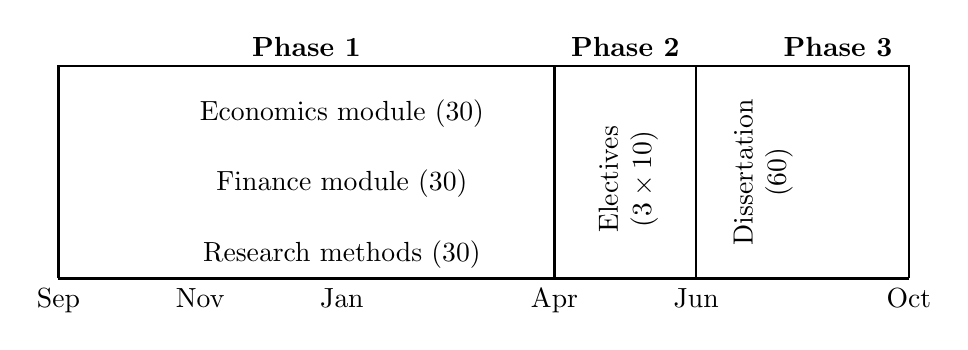
\begin{tikzpicture}[scale = 0.9]
%\draw [help lines] (0, 0) grid (12, 3);
\node [below] at (0, 0) {Sep};
\node [below] at (2, 0) {Nov};
\node [below] at (4, 0) {Jan};
\node [below] at (7, 0) {Apr};
\node [below] at (9, 0) {Jun};
\node [below] at (12, 0) {Oct};
\draw [very thick] (0, 0) -- (12, 0);
\draw [thick] (0,0) -- (0, 3) -- (7, 3) -- (7, 0);
\node [above] at (3.5, 3) {\textbf{Phase 1}};
%\node [above] at (3.5, 2) {ECM02};
%\node [above] at (3.5, 1) {FN};
%\node [above] at (3,5, 0) {OP394}; 
%\draw [thick] (2,0) -- (2, 3) -- (7, 3) -- (7, 0);
%\node [above] at (4.5, 3) {\textbf{Phase 2}};
\node [above] at (4.0, 2) {Economics module (30)};
\node [above] at (4.0, 1) {Finance module (30)};
\node [above] at (4.0, 0) {Research methods (30)};
\draw [thick] (7,0) -- (7, 3) -- (9, 3) -- (9, 0);
\node [above] at (8, 3) {\textbf{Phase 2}};
\node [above, rotate = 90, align = center] at (8.6, 1.4) {Electives\\($3\times10$)};
\draw [thick] (9,0) -- (9, 3) -- (12, 3) -- (12, 0);
\node [above] at (11, 3) {\textbf{Phase 3}};
\node [above, rotate = 90, align = center] at (10.5, 1.5) {Dissertation \\(60)};
\end{tikzpicture}
\end{frame}

\begin{frame}{Named degree}
MSc Finance and Investment is the core degree
\begin{itemize}[<+-| alert@+>]
\pause
\item You need 80 credits in other subjects to get finance and \dots
\item The dissertation and 2 of the 10 credit modules
\item For example \emph{Finance and Banking}
\begin{itemize}
\item Banking and financial institutions
\item Money, interest rates and banking
\item Dissertation in the area of banking
\end{itemize}
\end{itemize}
\end{frame}


\begin{frame}{Key issues}
Virtually all possibilities are in the course handbook.  However, there are three issues that tend to arise most often:
\begin{itemize}[<+-| alert@+>]
\pause
\item Correct referencing citation
\item Extensions 
\item Mitigating circumstances
\end{itemize}
\end{frame}

\begin{frame}{Correct referencing}
There are two rules: 
\pause
\begin{block}{}
Everything that is taken word-for-word \textbf{MUST} be put into quotation marks
\end{block}
\pause
\vspace{1cm}
\begin{block}{}
Ideas taken from other places \textbf{MUST} be referenced
\end{block}
\end{frame}

\begin{frame}{Referencing handbook}
\centering
\includegraphics[scale = 0.2]{"ref"}
\end{frame}


\begin{frame}{Extensions and mitigating circumstances}
You \textbf{MUST} submit your work before the deadline
\begin{itemize}[<+-| alert@+>]
\pause
\item If it is within 2 weeks of the deadline, it will be marked and you will receive feedback but it will be capped at 50\%. 
\item if it is after 2 weeks you will receive a mark of zero
\item If you have an illness or other emergency (see GEAR) you may apply for an \textbf{extension}
\item If you have an illness or other emergency that affects your work you may claim \textbf{mitigating circumstances}
\end{itemize}
\end{frame}

\begin{frame}{Failing assignments}
If you fail to achieve the \textbf{learning outcomes} on a piece of work
\begin{itemize}[<+-| alert@+>]
\pause
\item You will normally be allowed a \emph{referral}
\begin{itemize}
\item this will cap the work at 50
\end{itemize}
\item Mitigating circumstances may mean that you receive a \emph{deferral}
\begin{itemize}
\item this means the repeat is treated as the first attempt.  It is not capped. 
\end{itemize}
\end{itemize}
\end{frame}

\section{Induction week task}
\begin{frame}{Induction week task}
\begin{itemize}[<+-| alert@+>]
\pause
\item Work as a group
\item Present a summary of a finance question on Friday 30 September
\item Write an individual report (1000 words) due on Sunday 9 October
\item You will get \emph{formative feedback}
\item It allows you to know how you are doing
\item It allows me to see if you need help in particular areas
\end{itemize}
\end{frame}

\section{Working at Masters' level}
\begin{frame}{Moving to Masters}
There is an article on student from the University of Reading about Masters' level work
\begin{itemize}[<+-| alert@+>]
\pause
\item the workload is more intensive
\item the relationship with the tutors is different
\item there is an emphasis on application and critical thinking
\item you are an expert and should act in a professional manner
\item the aim is to become \textbf{an independent researcher}
\end{itemize}
\end{frame}

\begin{frame}{My own observations}
Three issues
\begin{itemize}[<+-| alert@+>]
\pause
\item Ability to adapt
\item Amount of work
\item Empirical nature of work
\end{itemize}
\end{frame}


\begin{frame}{Ability to adapt}
\begin{itemize}[<+-| alert@+>]
\item Don't just learn the answer
\item Lean the tool and know how to use them
\item Financial system and innovation
\item Importance of critical analysis
\end{itemize}
\end{frame}

\begin{frame}{Amount of work}
\begin{itemize}[<+-| alert@+>]
\item On the surface it may not look very much
\item Take the opportunity to read
\item Take a professional pride
\item Show that  you have \emph{master's level} ability analyse in a critical fashion
\end{itemize}
\end{frame}

\begin{frame}{Empirical side}
\begin{itemize}[<+-| alert@+>]
\item We live in a world of data
\item Data must be managed and presented
\item Data is the evidence to support the case that you make. 
\item Weekly exercises are important
\end{itemize}
\end{frame}



\end{document}



